\documentclass{article}
\usepackage[T1]{fontenc}
\usepackage{lmodern}
\usepackage{graphicx}
\usepackage{amsmath,amssymb}
\usepackage[a4paper,margin=2cm]{geometry}
\usepackage[absolute,overlay]{textpos}
\setlength{\TPHorizModule}{1mm}
\setlength{\TPVertModule}{1mm}
\usepackage[indonesian]{babel}
\usepackage{hyperref}
\setlength{\emergencystretch}{2em}
% unit: Halaman 22

\begin{document}

% === Halaman 22 (llm) ===

\begin{itemize}
  \item Steganografi di dalam film \textit{Mercury Rising} dan \textit{Beautiful Mind}
\end{itemize}

\vspace{10mm}

% deskripsi: Cuplikan layar dari film A Beautiful Mind yang menunjukkan karakter sedang berada di depan kaca dengan banyak coretan rumus matematika dan teks.
% bbox normalisasi: [0.1400, 0.2700, 0.4580, 0.8450]
\begin{textblock*}{66.78mm}(29.40mm,80.19mm)
\noindent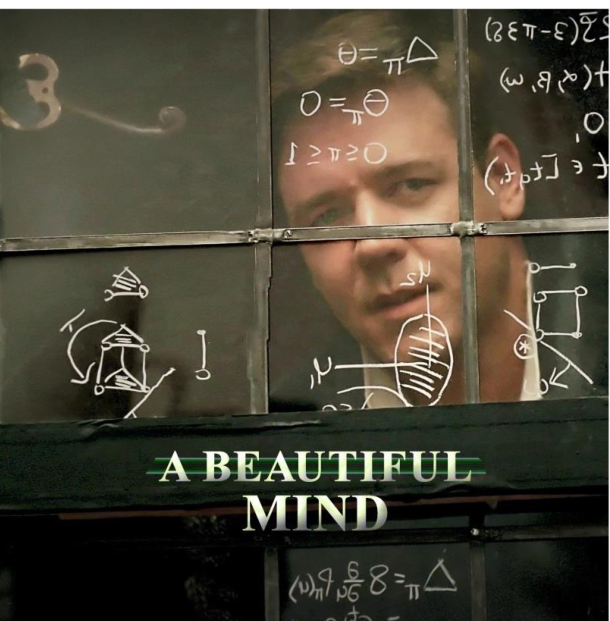
\includegraphics[width=66.78mm,height=170.77mm]{../../images/llm/page_022_img_01.png}%
\end{textblock*}

% deskripsi: Poster film Mercury Rising yang menampilkan Bruce Willis dan seorang anak kecil.
% bbox normalisasi: [0.5550, 0.2700, 0.7810, 0.8500]
\begin{textblock*}{47.46mm}(116.55mm,80.19mm)
\noindent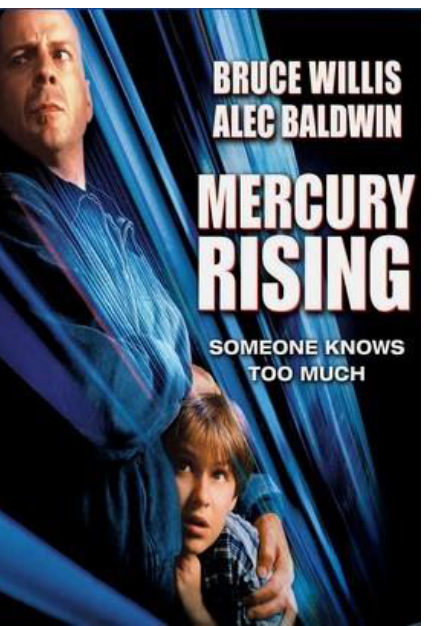
\includegraphics[width=47.46mm,height=172.26mm]{../../images/llm/page_022_img_02.png}%
\end{textblock*}

\end{document}
